% \subsection{背景介绍}
%@author: lhy
\subsubsection{ROS系统重要性}
人类生活与机器人密不可分。传统上,机器人在农业和制造业中被广泛用于任务自动化。最近的发展让机器人更加贴近每个人的日常生活。例如,亚马逊和谷歌正在部署无人配送系统[22,23],使用无人驾驶飞行器,机器人吸尘器的市场规模年增长率达到23\%[24],以及在2012年到2018年间,使用机器人进行手术的比例从2\%增加到15\%[25],显示出机器人产业为适应人类需求而快速增长的态势。同时,现代机器人,如自动驾驶车辆,正在变得更加复杂,要求集成复杂的子系统,例如感知、感觉、规划和执行。

为了应对开发复杂机器人系统的更高需求,机器人操作系统(ROS)[1]正在获得越来越多的关注。ROS是一个开源的中间件套件,用于机器人开发,它具有分布式机器人进程的消息传递机制、硬件抽象、广泛的开发工具(例如,模拟器)和机器人库(例如,路径规划算法)。使用ROS,开发者可以加速开发过程,无需重新发明轮子,而是可以专注于他们机器人的核心功能。凭借其多语言和多平台支持的理念,ROS正在成为机器人编程中的实际标准;它已被广泛采用于工业[26,27]、军事[28,29]、研究机构以及个人,预计到2024年将为55\%的商业机器人提供动力[30]。近些年ROS系统相关论文数量与Wiki用户数量如图1所示:

\begin{figure}[H]
  \centering
  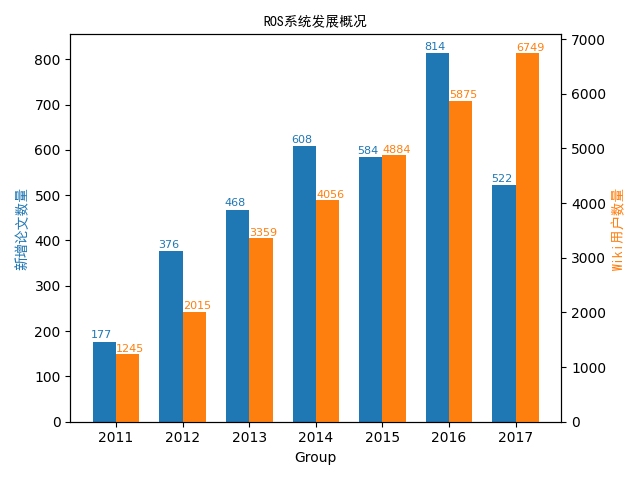
\includegraphics[width=0.8\textwidth]{ros_papers.png}
  \caption{ROS系统相关论文数量与Wiki用户数量}
\end{figure}

机器人操作系统(ROS)是一个开源平台,它为用C++和Python等不同语言实现机器人软件提供了许多实用的工具和库。超过740家商业公司正在使用ROS[2]来开发数百种实际应用的机器人[3],这表明了其在机器人开发中的流行度。然而,开发可靠的ROS程序具有挑战性,因为机器人可以在复杂的物理环境中工作,并可能遇到各种异常情况(如无效的配置参数和异常的传感器信息)。如果ROS程序不够可靠,它们的错误可能在与人类和其他机器人交互时导致危险事故。

ROS本身的缺陷或者开发者在应用中常用的ROS使用方式可能会影响依赖于ROS的广泛机器人系统,并对许多用户的安全和保障造成严重破坏。例如,ROS版本1没有认证的概念,允许网络上的任何实体完全访问任何机器人系统,窃听内部消息,甚至在知道IP地址和端口的情况下劫持执行。实际上,在互联网上扫描默认的ROS端口两个月后[31],发现部署在28个国家的超过100个ROS系统,这些系统完全暴露于此类攻击之下。ROS的最新版本(即ROS 2)在设计和实现时考虑了这些问题,并邀请了更广泛的公众对安全性进行审查。不幸的是,现有的工作和解决方案要么专注于关于认证和授权方法的网络安全方面[32,33,34,35],要么专注于回归测试[36],使得ROS社区在寻找影响机器人系统的健壮性和正确性的未知错误方面缺乏一种系统的测试方法。
\subsubsection{自动驾驶兴起与ROS}
自动驾驶技术的兴起标志着交通运输领域的一次重大革命,其不仅预示着交通安全、效率和环境影响的根本改进,而且还预示着个人出行和货物运输方式的深刻变革,而这一过程在很大程度上得益于机器人操作系统(Robot Operating System,ROS)的发展和应用。近年来,由于计算能力的显著提升、大数据技术的发展、人工智能算法的进步以及传感器技术的优化,自动驾驶汽车从理论研究和小规模试验逐步走向了公路测试和商业化应用的初步阶段。

根据国际汽车工程师学会(SAE)的定义[1],自动驾驶分为六个级别,从0级(无自动化)到5级(完全自动化)。目前,多数公开测试和部分商业化应用的自动驾驶汽车处于3级(有条件自动化)到4级(高度自动化)。尽管完全自动化(5级)的汽车尚未广泛部署,但多个技术开发者和制造商已经在进行相关的研发工作,并在不同国家和地区开展了路试。

随着自动驾驶技术的进步,对处理大量传感器数据、实现复杂决策逻辑和执行精确控制的需求不断增加,ROS的可扩展性和灵活性在此过程中显示出其不可或缺的价值。例如,ROS的消息传递系统支持多种编程语言,允许异构系统高效集成。此外,其庞大的开源社区贡献了大量的软件包,覆盖从3D视觉到路径规划等各种功能,极大地丰富了自动驾驶汽车的研发资源库。

经济学人智库的一份报告预测[2],到2035年,全球自动驾驶汽车的数量将达到近7500万辆。而麦肯锡公司的一项研究则估计[3],自动驾驶技术的全面部署将使交通事故造成的死亡人数减少90\%,同时还将大幅度提升道路运输效率和减少碳排放。图2展示了PRECEDENCE RESEARCH机构预测的未来自动驾驶市场规模:

\begin{figure}[H]
  \centering
  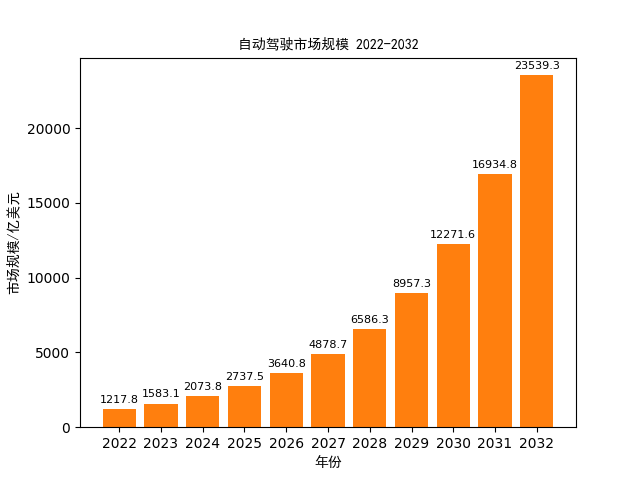
\includegraphics[width=0.8\textwidth]{market_size.png}
  \caption{自动驾驶市场规模}
  \label{fig:my_label}
\end{figure}

尽管自动驾驶技术的前景被广泛看好,但其商业化应用和普及还面临多重挑战,包括技术完善度、法律法规、道德伦理、消费者接受度以及基础设施配套等。例如,自动驾驶汽车在复杂的城市交通环境中的表现,以及在极端天气条件下的可靠性,仍然是技术研发中的重要挑战。

未来,随着相关技术的进一步成熟和相关政策的完善,自动驾驶汽车有望在更广泛的领域得到应用,从而实现对交通系统的根本性改造和优化。这将不仅影响交通运输本身,还将对城市规划、能源消费、环境保护以及人们的生活方式产生深远影响。

\subsubsection{自动驾驶产生漏洞的危害}
尽管自动驾驶汽车(AVs)承诺通过减少人为错误来增加道路安全,它们固有的技术漏洞却可能导致严重的安全后果。据国家公路交通安全管理局(NHTSA)估计,94\%的严重交通事故是由人为因素引起的,而自动驾驶技术的开发者们宣称,通过消除这一因素,可以极大地提高道路安全性[4]。然而,这种安全性的提升假设基于自动驾驶系统能够无缺陷地执行其预定任务,这在实践中往往难以实现。

自动驾驶汽车的技术漏洞主要分为两类:软件漏洞和硬件故障。软件漏洞包括但不限于算法错误、安全漏洞以及对异常情况的处理不足。硬件故障可能涉及传感器故障、执行机构的故障或其他关键组件的损坏。这些技术漏洞不仅可能导致单一车辆的操作失败,还可能对整个交通系统产生连锁反应,特别是在高度自动化和互联的交通环境中。

例如,2018年3月,在美国亚利桑那州发生了一起致命的自动驾驶汽车事故,一名行人在穿越街道时被一辆自动模式下的Uber汽车撞击,导致死亡。初步调查显示,该事故部分原因是系统无法正确识别并响应行人[5]。这一事件凸显了即使在自动驾驶技术取得显著进步的情况下,技术漏洞仍然可能导致灾难性后果。

此外,安全研究人员已经证明,自动驾驶汽车系统的安全漏洞可以被黑客利用,进而控制车辆的行驶方向或速度,造成严重安全威胁[6]。例如,通过篡改车辆的环境感知系统接收到的数据,攻击者可以使汽车忽略停车标志或其他关键交通信号,导致交通事故。

综上所述,尽管自动驾驶技术的发展被寄予厚望,能够在根本上改变我们的交通系统,降低事故率,提高交通效率,但技术漏洞的存在表明,要实现这些目标,还需要克服重大的技术和安全挑战。这要求汽车制造商、技术开发者、立法者和监管机构合作,不断提高自动驾驶系统的安全性和可靠性,同时为可能出现的技术漏洞和安全威胁制定全面的应对策略。

